\documentclass[../main.tex]{subfiles}
\graphicspath{{\subfix{../figures/}}}
%
\begin{document}
\section{策略模式(Strategy)}
策略模式属于对象形式的行为模式.其用意是针对一组算法,将每一个算法行为封装到具有共同接口的独立的类中,从而使得他们可以相互替换.策略模式使得算法可以在不影响到客户端的情况下发生变化.
%
\subsection{介绍}
\textbf{问题}:
假设现在要设计一个贩卖各类书籍的电子商务网站的购物车(Shopping Cart)系统.在计算价格时,一个最简单的实现就是把所有的货品的单价乘上数量,但是实际情况肯定比这要复杂.比如,网站可能对所有的教材类图书实行每本一元的折扣;对其余的图书没有折扣.对连环画类图书提供每本7%的促销折扣,而对非教材类的计算机图书有3%的折扣,对其余的图书没有折扣.由于有这样复杂的折扣算法,使得价格计算问题需要系统地解决.
那么怎么解决这个问题呢?

\textbf{解决方案}:
这里提供三种方案如下所示:
%
\begin{enumerate}
  \item 所有的业务逻辑都放在客户端里面.客户端利用条件选择语句决定使用哪一个算法.这样一来,客户端代码会变得复杂和难以维护.
  \item 客户端可以利用继承的办法在子类里面实现不同的行为,但是这样会使得类和行为紧密耦合在一起.强耦合会使两者不能单独演化.
  \item 使用策略模式.策略模式把行为和其应用环境割开来.环境类负责维护和查询策略类,各种算法则在具体策略类(ConcreteStrategy)中提供.
\end{enumerate}
%
\begin{itemize}
  \item 将算法和算法的使用环境(context)独立开来,使算法的增减、修改对其使用者透明.
  \item 策略模式正是解决这个问题的系统化方法.当出现新的促销折扣或现有的折扣政策出现变化时,只需要实现新的策略类,并被客户端使用即可.策略模式相当于``可插入式(Pluggable)的算法''.
  \item 当准备在一个系统里使用策略模式时,首先必须找到需要包装的算法,看看算法是否可以从使用环境中分割开来,最后再考察这些算法是否在以后发生变化.
\end{itemize}
%
\textbf{策略模式的用意}是针对一组算法,将每一个算法封装到具有共同接口的独立的类中,从而使得它们可以相互替换.策略模式使得算法可以在不影响到客户端的情况下发生变化.策略模式的简略类图如下所示.
%
\begin{figure}[H]
  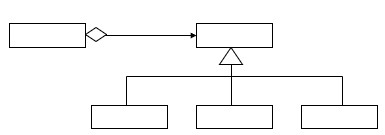
\includegraphics[width=0.35\textwidth]{27_1.jpg}
\end{figure}
%
\subsection{策略模式的结构}
策略又称做政策(Policy)模式.下面是一个示意性的策略模式结构图:
%
\begin{figure}[H]
  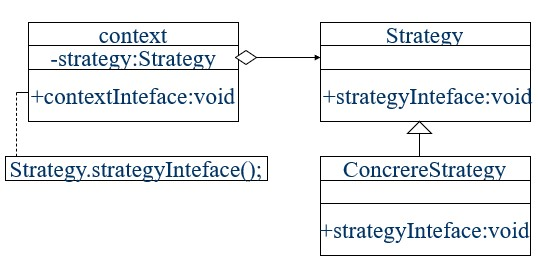
\includegraphics[width=0.45\textwidth]{27_2.jpg}
\end{figure}
%
\textbf{模式涉及到三个角色}:
\begin{itemize}
  \item 环境(Context)角色:表示策略的使用环境,它持有一个Strategy对象的引用.
  \item 抽象策略(Strategy)角色:这是一个抽象角色,通常由一个接口或抽象类实现.此角色给出所有的具体策略类所需的接口.
  \item 具体策略(ConcreteStrategy)角色:包装了相关的算法或行为.
\end{itemize}
%
\lstinputlisting[language=java]{./code/27/1/Context.java}
\lstinputlisting[language=java]{./code/27/1/Strategy.java}
\lstinputlisting[language=java]{./code/27/1/ConcreteStrategy.java}
%
这里所给出的仅仅是策略模式的最简单实现,因此具体策略角色才只有一个.一般而言,有意义的策略模式的应用都会涉及到多个的具体策略角色.我们可以把这里给出的源代码当作策略模式的骨架,在将它使用到自己的系统中时,还需要添加上与系统有关的逻辑.
%
\subsection{例:Java语言内部的例子}
\noindent Java语言使用了很多的设计模式,包括策略模式.使用策略模式的例子可以在java.awt库和Swing库中看到.

\textbf{AWT中的LayoutManager}:
java.awt类库需在运行期间动态地由客户端决定一个Container对象怎样排列它所有的GUI构件.Java语言提供了几种不同的排列方式,包装在不同的类里:
BorderLayout,FlowLayout,GridBagLayout,GridLayout,CardLayout.

LayoutManager的类图如下所示:
%
\begin{figure}[H]
  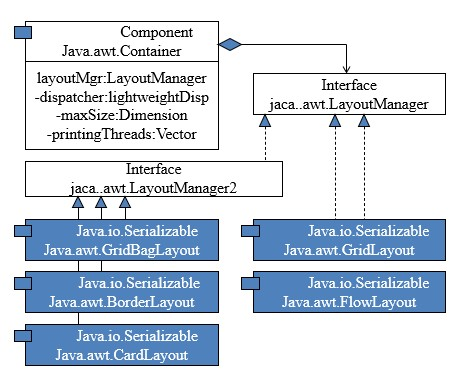
\includegraphics[width=0.60\textwidth]{27_3.jpg}
\end{figure}
%
图中没有阴影部分的类是具体策略角色,java.awt.Container类是环境角色,而java.awt.LayoutManager则是抽象策略角色.
任何人都可以设计实现自己的Layout类.比如Borland公司就在Jbuilder里面提供了XYLayout,作为对几种JDK提供的Layout类的补充.

\textbf{系统涉及到三个角色}:
%
\begin{itemize}
  \item 环境角色:在这里由Container类扮演.
  \item 抽象策略(Strategy)角色:这是一个抽象角色,由LayoutManger类扮演.此角色给出所有的具体Layout类所需要的接口.
  \item 具体策略(ConcreteStrategy)角色:由BorderLayout、FlowLayout、GridLayout、GridLayout、GridBagLayout、CardLayout等扮演(请见图中没有阴影的类),他们包装了不同的Layout行为.
\end{itemize}
%
\subsection{例:排序策略系统}
\noindent 假设要设计一个排序系统,可以动态地使用二元排序、堆栈排序、快速排序、基数排序等排序算法.
显然,采用策略模式把几种排序算法包装到不同的算法类里面,让所有的算法类具有相同的接口,就是一个很好的设计.排序策略系统的设计如下图所示.
%
\begin{figure}[H]
  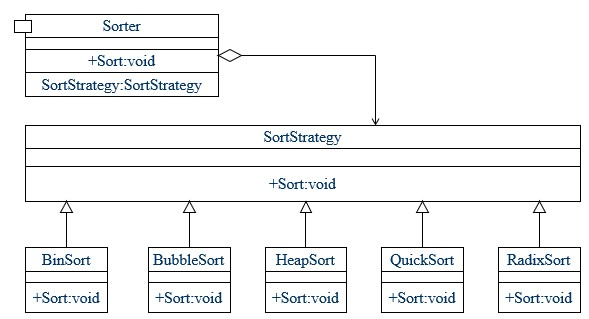
\includegraphics[width=0.60\textwidth]{27_4.jpg}
\end{figure}
%
\noindent 客户端/环境类必须决定在何时使用哪个排序算法,即这个决定不是在模式内部决定的.
%
\subsection{例:图书折扣的计算}
\lstinputlisting[language=java]{./code/27/2/DiscountStrategy.java}
\lstinputlisting[language=java]{./code/27/2/NoDiscountStrategy.java}
\lstinputlisting[language=java]{./code/27/2/FlatRateStrategy.java}
\lstinputlisting[language=java]{./code/27/2/PercentageStrategy.java}
\lstinputlisting[language=java]{./code/27/2/Book.java}
%
\subsection{使用场景}
在下面的情况下应当考虑使用策略模式:
%
\begin{enumerate}
  \item 如果在一个系统里面有许多类,它们之间的区别仅在于它们的行为,那么策略模式可以动态地让一个对象在许多行为中选择一种行为.
  \item 一个系统需要动态地在几种算法中选择一种.那么这些算法可以包装到一个个地具体算法类里面,而这些具体算法类都是一个抽象算法的子类.换言之,这些具体算法均有统一的接口,由于多态性原则,客户端可以选择使用任何一个具体算法类,并只持有一个数据类型是抽象算法类的对象.
  \item 一个系统的算法使用的数据不可以让客户端知道.策略模式可以避免让客户端涉及到不必要接触到的复杂的和只与算法有关的数据.
  \item 如果一个对象有很多的行为,如果不用恰当的模式,这些行为就只好使用多重的条件选择语句来实现.此时,使用策略模式,把这些行为转移到相应的具体策略类里面,就可以避免使用难以维护的多重条件选择语句,并体现面向对象设计的概念.
\end{enumerate}
%
\textbf{策略模式与其他模式的关系}:
策略模式与很多其它的模式都有着广泛的联系.Strategy很容易和Bridge模式相混淆.虽然它们结构很相似,但它们却是为解决不同的问题而设计的.Strategy模式注重于算法的封装,而Bridge模式注重于分离抽象和实现,为一个抽象体系提供不同的实现.Bridge模式与Strategy模式都很好的体现了"Favor composite over inheritance"的观点.

\textbf{设计原则的讨论}:
策略模式是开闭原则的一个极好的应用范例.
在采用策略模式之前,设计师必须从``开-闭原则''出发,考察这个图书销售系统是否有可能在将来引入新的折扣算法.如果有可能,那么就应当将所有的折扣算法封装起来,因为他们是可变化的因素.
%
\end{document}
